\documentclass{standalone}

\usepackage{amsmath}
\usepackage{tikz}
\usetikzlibrary{arrows.meta, positioning, calc, }

\begin{document}

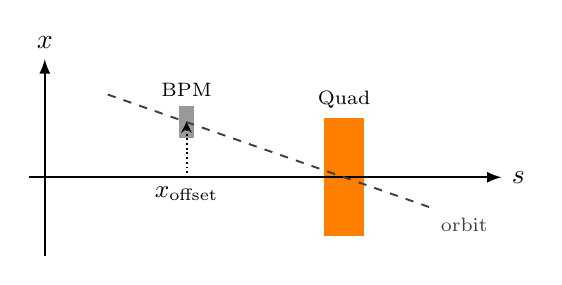
\begin{tikzpicture}[>=latex]
    \coordinate (O) at (0, 0);
    \coordinate (B) at (-2, 0.7);

    \pgfmathsetmacro{\qlarg}{0.5}   
    \pgfmathsetmacro{\qalt}{1.5}
    \pgfmathsetmacro{\blarg}{0.2}
    \pgfmathsetmacro{\balt}{0.4}

  % Quadrupole laranja (Correção no '+')
    \path[fill=orange, draw=none] ($(O)+(\qlarg/2,\qalt/2)$) rectangle ($(O)-(\qlarg/2,\qalt/2)$);
    \node[above] at ($(O)+(0,\qalt/2)$) {\scriptsize Quad};
    
    % BPM cinza (Correção no '+')
    \path[fill=black!40, draw=none] ($(B)+(\blarg/2,\balt/2)$) rectangle ($(B)-(\blarg/2,\balt/2)$);
    \node[above] at ($(B)+(0,\balt/2)$) {\scriptsize BPM};
    
    \draw[thick, ->] (-4, 0) -- (2, 0) node[right] {$s$};
    \draw[thick, ->] (-3.8, -1) -- (-3.8, 1.5) node[above] {$x$};

    \draw[line width=0.7pt, darkgray, dashed] ($1.5*(B)$) -- ($-0.55*(B)$) node[below right, darkgray] {\scriptsize orbit};

    \draw[line width=0.7pt, black, stealth-, densely dotted] (B) -- (-2, 0);
    \node[below] at (-2, 0) {\small $x_\text{offset}$};

\end{tikzpicture}


\end{document}